\documentclass[12pt,letterpaper]{article}

% just for the example
\usepackage{lipsum}
% Set margins to 1.5in
\usepackage[margin=1.5in]{geometry}

% for graphics
\usepackage{graphicx}
\graphicspath{{./figures/}}

% for crimson text
\usepackage{crimson}
\usepackage[T1]{fontenc}

% setup parameter indentation
\setlength{\parindent}{0pt}
\setlength{\parskip}{6pt}

% for 1.15 spacing between text
\renewcommand{\baselinestretch}{1.15}

% For defining spacing between headers
\usepackage{titlesec}
% Level 1
\titleformat{\section}
  {\normalfont\fontsize{18}{0}\bfseries}{\thesection}{1em}{}
% Level 2
\titleformat{\subsection}
  {\normalfont\fontsize{14}{0}\bfseries}{\thesection}{1em}{}
% Level 3
\titleformat{\subsubsection}
  {\normalfont\fontsize{12}{0}\bfseries}{\thesection}{1em}{}
% Level 4
\titleformat{\paragraph}
  {\normalfont\fontsize{12}{0}\bfseries\itshape}{\theparagraph}{1em}{}
% Level 5
\titleformat{\subparagraph}
  {\normalfont\fontsize{12}{0}\itshape}{\theparagraph}{1em}{}
% Level 6
\makeatletter
\newcounter{subsubparagraph}[subparagraph]
\renewcommand\thesubsubparagraph{%
  \thesubparagraph.\@arabic\c@subsubparagraph}
\newcommand\subsubparagraph{%
  \@startsection{subsubparagraph}    % counter
    {6}                              % level
    {\parindent}                     % indent
    {12pt} % beforeskip
    {6pt}                           % afterskip
    {\normalfont\fontsize{12}{0}}}
\newcommand\l@subsubparagraph{\@dottedtocline{6}{10em}{5em}}
\newcommand{\subsubparagraphmark}[1]{}
\makeatother
\titlespacing*{\section}{0pt}{12pt}{6pt}
\titlespacing*{\subsection}{0pt}{12pt}{6pt}
\titlespacing*{\subsubsection}{0pt}{12pt}{6pt}
\titlespacing*{\paragraph}{0pt}{12pt}{6pt}
\titlespacing*{\subparagraph}{0pt}{12pt}{6pt}
\titlespacing*{\subsubparagraph}{0pt}{12pt}{6pt}

% Set caption to correct size and location
\usepackage[tableposition=top, figureposition=bottom, font=footnotesize, labelfont=bf]{caption}

% set page number location
\usepackage{fancyhdr}
\fancyhf{} % clear all header and footers
\renewcommand{\headrulewidth}{0pt} % remove the header rule
\rhead{\thepage}
\pagestyle{fancy}

% Overwrite Title
\makeatletter
\renewcommand{\maketitle}{\bgroup
   \begin{center}
   \textbf{{\fontsize{18pt}{20}\selectfont \@title}}\\
   \vspace{10pt}
   {\fontsize{12pt}{0}\selectfont \@author} 
   \end{center}
}
\makeatother

% Used for Tables and Figures
\usepackage{float}

% For using lists
\usepackage{enumitem}

% For using APA Citation format
\usepackage{apacite}

% Custom Quote
\newenvironment{myquote}[1]%
  {\list{}{\leftmargin=#1\rightmargin=#1}\item[]}%
  {\endlist}
  
% Create Abstract 
\renewenvironment{abstract}
{\vspace*{-.5in}\fontsize{12pt}{12}\begin{myquote}{.5in}
\noindent \par{\bfseries \abstractname.}}
{\medskip\noindent
\end{myquote}
}

\begin{document}

% Set Title, Author, and email
\title{Assignment M1}
\author{Snejana Shegheva \\ sshegheva3@gatech.edu}

\maketitle
\thispagestyle{fancy}

\begin{abstract}
Mapping data from one form to another for its ease-of-use is at the core of the \textit{Extract, Transform and Load} process. There exist many tools that can accomplish the task of creating and maintaining a data warehouse. However, sometimes it is advantageous to have a custom solution that allows user to interact with the data directly during some or all of the ETL phases. In this project, we analyze an internal interface of a \textit{transform} task that prepares the data for use in a personalized recommendation system powered by Artificial Intelligence engines. 
\end{abstract}

\subsection*{Problem Space}
The data ingestion is described by the \textit{Extract, Transform and Load} (ETL) process - a cycle that converts a raw data into structured records more convenient for further Data Analysis and/or use for Machine Learning algorithms \cite{wiki:xxx}. Figure~\ref{fig::1} shows the ETL process from the Source to the Destination. The entire cycle may be completely hidden from the user (full automation of data ingestion), or a human is required to guide the components of the process to reach their desired goal. In this project we focus on the \textit{transform} task that is centered around interactions with the user to alter the original data to meet their needs. For example, a user who looks at the weather feed in Fahrenheit may choose to convert it to Celsius. 

\begin{figure}[H]
\centering
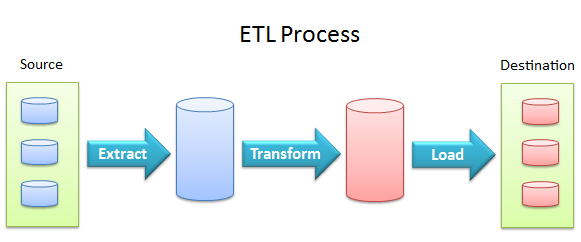
\includegraphics[width=3in, scale=.3]{ETLProcess.png}
\caption{Extract-Transform-Load Process from Data Science Central blogpost on Open Source ETL tools (https://www.datasciencecentral.com/profiles/blogs/10-open-source-etl-tools)}
\label{fig::1}
\end{figure}

To accomplish the data transformation task, a user needs an access to the original data, as well as an arsenal of mapping tools suitable to the domain. Figure~\ref{fig::2} shows an existing version of an internal interface \footnote{A very rough version of a custom tool to perform user-driven ETL process.} that we will be analyzing and re-designing to improve user experience in undertaking the transformation task. 

\begin{figure}[H]
\centering
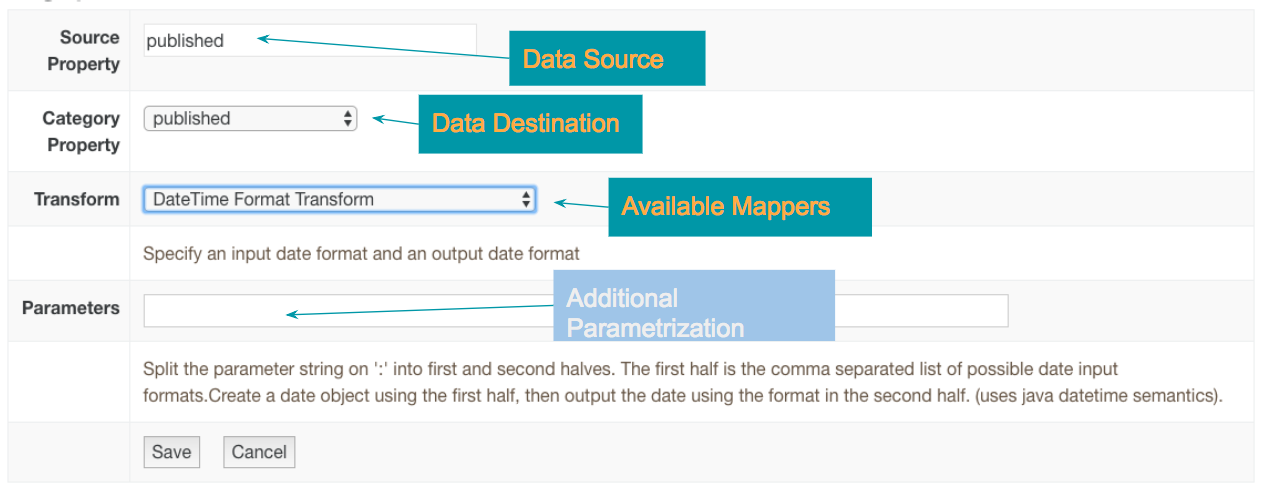
\includegraphics[width=4in, scale=.4]{NaraTransform.png}
\caption{A version of an internal interface for transforming a single data field. Here, the data source is the data from the Arxiv Library collected via ATOM API. User selects the original field, here the \textit{published} date, and wishes to transform it to a different date format.}
\label{fig::2}
\end{figure}

Our main goal is to assess all the weak areas of the existing interface in order to provide recommendations for alternative models that simplify the user interaction without assuming any pre-existing knowledge of the tool.

\subsection*{User Types}
Let's outline the user who is expected to engage in the data transformation task described above. The target user's expertise ranges from a novice (an external business client without extensive technical background) to an expert (data analyst interacting with the tool on daily basis). The task assumes a basic proficiency with computer interfaces, which is a reasonable assumption given that the expected audience are professionals that use data to make business decisions. The task for different categories of users remains the same, however, the approach for accomplishing it may differ significantly. On one hand, a user with substantial knowledge of the data (a domain expert) may want to explore complex relationships between the existing variables and generate new outcomes that capture the essence of the observed relationship. On the other hand, a user tasked with a data cleanup process, might not wish to delve into data intricacies, and instead focus on common exercise of standardizing the content (for example, change a \textit{thousands} separator in the numerical data). 

A context of the task varies significantly, and is largely data-driven. A system for recommending movies involves data on user preferences and feedback. A system for optimizing financial portfolios continuously streams data from financial markets and/or other sources. Therefore, an interface for accomplishing the described goals should be domain agnostic, and abstract the functionality of the transformation process to support a plethora of contexts. In general, a user needs an access to a Web interface that allows uploading a data from many sources, and subsequently either loading it to warehouse as is, or applying necessary and desired transformations to alter the original form. In order to accomplish a transformation task, users needs to 1) know \textit{what} data and in what form is currently available, 2) define the rules to \textit{convert} the data from the original to the desired form, 3) \textit{see} the final result to confirm the success, or \textit{receive a feedback} for required adjustments in failure cases. The large bulk of the user interaction with the interface is expected around the sub-task of defining a transformation rule. Therefore, a good design should focus on simplifying this step by providing an intuitive interface for data manipulation.


\subsection*{Needfinding Plan 1 - Hacks and Workarounds}
We have briefly described what is the user's ultimate goal, and how that can be broken down into sub-goals. In this section, we are going to further zoom into the user's actions for performing the task of data transformation. As our objective is to understand the weaknesses of the existing interface, as shown in Figure~\ref{fig::2}, we analyze the cases where the user breaks out of the provided interface and resorts to various hacks and workarounds to accomplish the task. A user in a Data Scientist role has a frequent need for manipulating the raw data that moves through the ETL pipeline. The main reasons for why the user in that role currently changes their intended workflow and perform a subsets of the actions outside of the given interface can be summarized by the following three categories: 

\begin{enumerate}
    \item \textbf{Limited functionality}. Prior to deciding on the transformation rules, user needs to have a visibility on the data being transformed. In the current interface (see Figure~\ref{fig::3}), user selects the targeted data field, for example a \textit{published date}, and is given an \textit{edit} button. However, the interface does not provide enough information to make a fully informed action on the required transformation rule. Therefore, a workaround\#1:  
    \subparagraph{Load the data in the external interface (command line, Jupyter notebooks, database queries) to explore descriptive statistics of the original field - the most frequent values,  the extreme values, etc.}
    
    \begin{figure}[H]
    \centering
    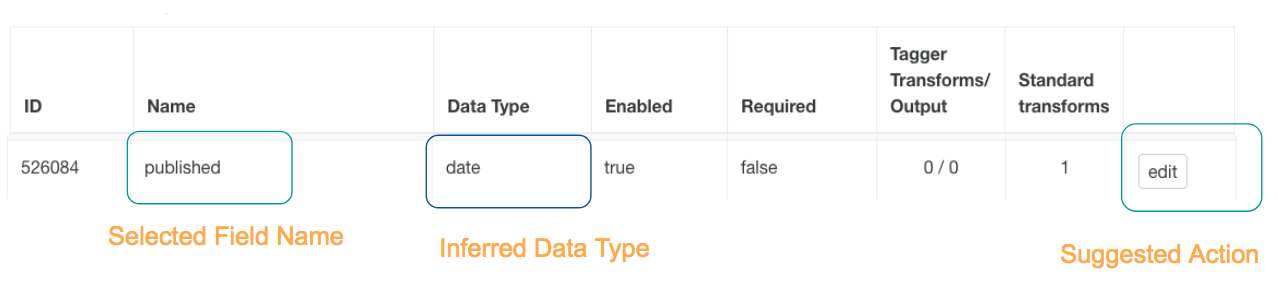
\includegraphics[width=4in, scale=.4]{DataVisibility.png}
    \caption{An example of the interface limitation to provide the user with knowledge of the present data form to enable an informed action.}
    \label{fig::3}
    \end{figure}
    
    
    \item \textbf{Poor Organization}. After the user has decided on transformation rule, the next step is to map the intentions to the given selection
\end{enumerate}

\subsection*{Needfinding Plan 2}
\lipsum[1]

\subsection*{Needfinding Plan 3}
\lipsum[1]


\bibliographystyle{apacite} 
\bibliography{bibtemp}

\end{document}
